\documentclass[11pt, a4paper]{article}

% ==================== PAQUETES ====================
\usepackage[utf8]{inputenc}
\usepackage[T1]{fontenc}
\usepackage[spanish]{babel}
\usepackage[margin=2.3cm]{geometry}
\usepackage{amsmath, amssymb}
\usepackage{array, booktabs, tabularx}
\usepackage{xcolor}
\usepackage{graphicx}
\usepackage{tikz}
\usepackage{hyperref}
\usepackage{fancyhdr}
\usepackage{enumitem}
\usepackage{titlesec}
\usepackage{tcolorbox}
\usepackage{longtable}

\usetikzlibrary{shapes, arrows, positioning, calc, trees, fit}
\tcbuselibrary{skins, breakable}

% ==================== COLORES ====================
\definecolor{policiaAzul}{HTML}{0A3B66}
\definecolor{policiaAzulClaro}{HTML}{1E5A8E}
\definecolor{policiaDorado}{HTML}{C9A227}
\definecolor{grisClaro}{HTML}{F4F6F8}
\definecolor{grisBorde}{HTML}{DCE2E8}
\definecolor{acentoSuave}{HTML}{EAF2FA}
\definecolor{exitoVerde}{HTML}{1E7E34}
\definecolor{exitoSuave}{HTML}{E9F7EF}
\definecolor{alertaRojo}{HTML}{C0392B}
\definecolor{alertaSuave}{HTML}{FDECEA}
\definecolor{causa}{HTML}{A93226}
\definecolor{consecuencia}{HTML}{7D3C98}

% ==================== ESTILO ====================
\hypersetup{
  colorlinks=true,
  linkcolor=policiaAzul,
  urlcolor=policiaAzulClaro,
  pdftitle={Guia Demuestro mi aprendizaje U1 (Partes I y II) - Matematica aplicada},
  pdfauthor={Jose Javier Mercado Reyes - ESJIM}
}

\titleformat{\section}[hang]
  {\Large\bfseries\color{policiaAzul}}
  {\thesection.}{0.6em}{}
  [\vspace{4pt}{\color{policiaDorado}\titlerule[1.2pt]}]

\titlespacing*{\section}{0pt}{1.8em}{0.9em}

\titleformat{\subsection}[hang]
  {\large\bfseries\color{policiaAzulClaro}}
  {\thesubsection.}{0.5em}{}

\titlespacing*{\subsection}{0pt}{1.2em}{0.5em}

% Encabezado/pie
\pagestyle{fancy}
\fancyhf{}
\fancyhead[L]{\footnotesize\color{policiaAzul}\textbf{ESJIM} $\cdot$ Matem\'atica aplicada a la profesi\'on}
\fancyhead[R]{\footnotesize\color{policiaAzul}U1 $\cdot$ Demuestro mi aprendizaje I y II}
\fancyfoot[C]{\footnotesize\color{policiaAzul}P\'agina \thepage\ de \pageref*{LastPage}}
\renewcommand{\headrulewidth}{0.4pt}
\renewcommand{\headrule}{\color{policiaDorado}\hrule width\headwidth height0.8pt}
\usepackage{lastpage}

% Cajas tem\'aticas
\newtcolorbox{cajaInfo}[1][]{
  colback=acentoSuave, colframe=policiaAzulClaro,
  fonttitle=\bfseries\color{white}, title=#1,
  arc=2mm, left=10pt, right=10pt, top=6pt, bottom=6pt,
  breakable
}
\newtcolorbox{cajaExito}{
  colback=exitoSuave, colframe=exitoVerde, coltitle=exitoVerde,
  arc=2mm, left=10pt, right=10pt, top=6pt, bottom=6pt,
  leftrule=4pt, rightrule=0pt, toprule=0pt, bottomrule=0pt,
  breakable
}
\newtcolorbox{cajaAlerta}{
  colback=alertaSuave, colframe=alertaRojo, coltitle=alertaRojo,
  arc=2mm, left=10pt, right=10pt, top=6pt, bottom=6pt,
  leftrule=4pt, rightrule=0pt, toprule=0pt, bottomrule=0pt,
  breakable
}
\newtcolorbox{cajaPaso}[1][]{
  colback=white, colframe=policiaDorado, coltitle=policiaAzul,
  fonttitle=\bfseries, title=#1,
  arc=2mm, left=10pt, right=10pt, top=6pt, bottom=6pt,
  leftrule=4pt, rightrule=0.4pt, toprule=0.4pt, bottomrule=0.4pt,
  breakable
}

% ==================== DOCUMENTO ====================
\usepackage{multirow}
\newcommand{\var}[1]{\texttt{\small #1}}
\newtcolorbox{cajaModelo}[1][]{
  colback=grisClaro, colframe=policiaAzul, coltitle=white,
  fonttitle=\bfseries, title=#1,
  arc=2mm, left=10pt, right=10pt, top=6pt, bottom=6pt, breakable
}
\setlength{\parskip}{4pt}
\setlength{\emergencystretch}{3em}


\begin{document}

% ===================================================== PORTADA
\begin{titlepage}
\centering
\vspace*{1.2cm}

\begin{tcolorbox}[colback=policiaAzul, colframe=policiaDorado, boxrule=2pt, arc=4mm, left=20pt, right=20pt, top=20pt, bottom=20pt]
\color{white}
{\footnotesize\textbf{ESCUELA DE SUBOFICIALES Y NIVEL EJECUTIVO}}\\[2pt]
{\footnotesize ``GONZALO JIMÉNEZ DE QUESADA''}\\[10pt]
\color{policiaDorado}\rule{0.4\textwidth}{0.6pt}\\[10pt]
\color{white}
{\LARGE\textbf{Guía orientadora}}\\[6pt]
{\Large \textit{Demuestro mi aprendizaje --- Partes I y II}}\\[10pt]
\color{policiaDorado}
{\large\textbf{Unidad 1}}\\[3pt]
\color{white}
{\large Modelos Matemáticos para una Gestión Policial Eficiente}\\[6pt]
{\normalsize Optimización de Recursos y Análisis de Estadísticas Delictivas}\\
{\normalsize en la Administración Policial}\\[14pt]
\color{policiaDorado}\rule{0.4\textwidth}{0.6pt}\\[10pt]
\color{white}
{\normalsize Matemática aplicada a la profesión}
\end{tcolorbox}

\vspace{1cm}

\begin{tabular}{@{}p{0.25\textwidth}p{0.65\textwidth}@{}}
\textbf{\color{policiaAzul}Docente:} & José Javier Mercado Reyes\\[5pt]
\textbf{\color{policiaAzul}Asignatura:} & 338-ADMI-MATE-2 Matemática aplicada a la profesión\\[5pt]
\textbf{\color{policiaAzul}Secciones:} & 018457 $\cdot$ 018458 $\cdot$ 018459\\[5pt]
\textbf{\color{policiaAzul}Actividades:} & Demuestro mi aprendizaje Parte I y Parte II (colaborativas)\\[5pt]
\textbf{\color{policiaAzul}Apertura:} & Jueves 22 de octubre de 2026, 00:01\\[5pt]
\textbf{\color{policiaAzul}Cierre:} & Domingo 20 de diciembre de 2026, 23:59\\[5pt]
\textbf{\color{policiaAzul}Valor:} & 5,00 puntos cada parte, calificadas con rúbrica
\end{tabular}

\vfill

\begin{cajaInfo}[\textbf{Propósito de esta guía}]
Esta guía acompaña las dos entregas de \textbf{Demuestro mi aprendizaje} de la Unidad 1.
Reúne en un solo documento lo que la rúbrica exige, cómo trabajar con las bases de datos
del aula y un \textbf{catálogo de dieciocho modelos matemáticos resueltos paso a paso con los
datos reales} de las bases BD1, BD2 y BD3: desde la estadística descriptiva, Pareto y la
probabilidad, pasando por Poisson, la binomial, intervalos de confianza, chi-cuadrado,
ANOVA, regresión lineal y logística y series de tiempo, hasta la programación lineal,
la teoría de colas, la simulación Monte Carlo, K-Means y las cadenas de Markov.

\textbf{Cómo usarla:} los ejemplos muestran el procedimiento completo. Su grupo debe
\textbf{formular su propio problema}, elegir otra combinación de variables, delitos,
localidades o ciudades, y aplicar al menos tres de los modelos. Copiar los ejemplos tal
cual no cumple la actividad.
\end{cajaInfo}

\vspace{0.4cm}
{\footnotesize \color{policiaAzul} Periodo 2026-III}
\end{titlepage}

\tableofcontents
\newpage

% ===================================================== 1
\section{Qué se espera de usted}

\subsection{Objetivo de las actividades}
\begin{cajaInfo}[\textbf{Objetivo}]
Aplicar modelos matemáticos ligados al análisis estadístico, la optimización y la
representación gráfica de datos en el contexto policial, para mejorar la planificación,
la distribución de recursos y la resolución de problemas operativos de manera efectiva y
fundamentada.
\end{cajaInfo}

Las dos partes forman \textbf{un mismo proyecto}. En la Parte I su grupo define un
problema, procesa los datos y aplica modelos. En la Parte II interpreta lo encontrado,
extrae patrones y lo convierte en un \textbf{plan operativo} con conclusiones y
recomendaciones. Lo que haga bien en la Parte I es la base de la Parte II.

\subsection{Las dos entregas de un vistazo}

\begin{center}
\footnotesize
\begin{tabularx}{\textwidth}{@{}p{3.1cm}XX@{}}
\toprule
& \textbf{Parte I} & \textbf{Parte II}\\
\midrule
Propósito & Definir el proyecto, procesar los datos y aplicar modelos & Interpretar resultados, extraer patrones y formular el plan operativo\\[3pt]
Extensión & 5 a 7 páginas o diapositivas & 8 a 10 páginas o diapositivas\\[3pt]
Contenido obligatorio & Introducción $\cdot$ Datos y análisis $\cdot$ Modelos matemáticos aplicados $\cdot$ Gráficos & Todo lo de la Parte I (mejorado) $+$ Resultados (patrones) $+$ Plan operativo $+$ Conclusiones y recomendaciones\\[3pt]
Criterios de la rúbrica & Análisis de datos (1,5) $\cdot$ Representación gráfica (1,5) $\cdot$ Redacción y estructura (1,0) $\cdot$ Uso de herramientas estadísticas (1,0) & Interpretación de resultados (1,5) $\cdot$ Representación gráfica (1,5) $\cdot$ Planificación, conclusiones y recomendaciones (1,0) $\cdot$ Redacción y estructura (1,0)\\[3pt]
Formato & \multicolumn{2}{l}{PDF, diseño visual, poco texto, gráficos de alta calidad, datos institucionales en la portada}\\
\bottomrule
\end{tabularx}
\end{center}

\begin{cajaAlerta}
\textbf{Trabajo colaborativo.} Ambas partes se desarrollan en el grupo de trabajo que
eligió en la plataforma. \textbf{Cada integrante debe subir el archivo} y la portada debe
llevar el \textbf{nombre completo de todos los integrantes}. Un documento con la palabra
``Grupo 1'' y sin nombres no permite identificar a los autores.
\end{cajaAlerta}

% ===================================================== 2
\section{Las bases de datos del aula}

El docente dejó en el aula tres bases académicas en Excel. \textbf{Su informe debe
trabajar con una o más de ellas}; no se aceptan datos inventados, ``simulados'' o
``ilustrativos''. Todas tienen 250 registros y una hoja \textit{Guía de Variables} que
sugiere modelos para cada variable.

\begin{center}
\footnotesize
\begin{tabularx}{\textwidth}{@{}p{2.6cm}p{4.6cm}X@{}}
\toprule
\textbf{Base} & \textbf{Variables clave} & \textbf{Preguntas que permite responder}\\
\midrule
\textbf{BD1} Incidentes delictivos Bogotá (ene-2024 a jun-2025, 12 localidades) &
\var{Fecha, Hora, Día\_Semana, Tipo\_Delito, Localidad, Latitud, Longitud, Arma\_Medio, Edad\_Víctima, Tiempo\_Respuesta\_Min, Captura} &
¿Dónde, cuándo y cómo se concentra el delito? ¿Cuánto tarda la respuesta? ¿Qué factores se asocian con la captura? ¿Cuántos casos esperar por mes?\\[4pt]
\textbf{BD2} Gestión de cuadrantes (Bogotá, Medellín, Cali, Barranquilla; ago--oct 2024) &
\var{Ciudad, Estación, Cuadrante, Área\_km2, Población\_Cuadrante, Policías\_Asignados, Patrullas\_Disponibles, Motos\_Disponibles, Turno, Llamadas\_123, Incidentes\_No\_Atendidos, Tiempo\_Respuesta\_Prom\_Min, Capturas, Costo\_Operativo\_COP} &
¿Cómo rinden los recursos? ¿Qué relación hay entre patrullas y tiempo de respuesta? ¿Cómo redistribuir el personal y los vehículos? ¿Cuánto cuesta cada resultado?\\[4pt]
\textbf{BD3} Perfil criminal y reincidencia &
\var{Edad\_Captura, Nivel\_Educativo, Estrato, Delito\_Principal, Antecedentes\_Previos, Pertenece\_Banda, Programa\_Resocialización, Reincidió, Puntaje\_Riesgo} &
¿Qué características se asocian con la reincidencia? ¿Funciona la resocialización? ¿Cómo se mueve un individuo entre estados (cadena de Markov)?\\
\bottomrule
\end{tabularx}
\end{center}

\begin{cajaExito}
\textbf{Antes de calcular, depure.} Verifique que no haya registros vacíos ni duplicados
(en BD1 hay 250 identificadores únicos) y anote el periodo que cubre la base. En BD1,
2024 tiene 12 meses (172 registros) y 2025 solo el primer semestre (78 registros):
\textbf{no compare totales anuales} como si fueran periodos iguales. Diga siempre cuántos
registros usó ($n$) y use ese mismo $n$ en todo el informe.
\end{cajaExito}

% ===================================================== 3
\section{Parte I --- Fase 1: definir el proyecto}

Un buen informe empieza por una pregunta clara. Antes de abrir Excel, el grupo debe
redactar cuatro elementos:

\begin{cajaPaso}[\textbf{1. Problema central}]
Una frase concreta, ubicada en el territorio y en el tiempo, y medible con la base.
\par\smallskip
\textit{Débil:} ``La inseguridad afecta a la ciudad''.\par
\textit{Bien formulado:} ``En la muestra BD1 (250 incidentes, Bogotá, ene-2024 a
jun-2025) el tiempo medio de respuesta es de 12,49 minutos y en tres localidades supera
los 15 minutos, lo que reduce la posibilidad de captura en flagrancia''.
\end{cajaPaso}

\begin{cajaPaso}[\textbf{2. Preguntas de investigación (3 a 5)}]
Cada pregunta debe poder responderse con un modelo. Ejemplos:
\begin{itemize}[leftmargin=1.4em,itemsep=1pt]
\item ¿Cómo se distribuye el tiempo de respuesta y qué tan disperso es? $\rightarrow$ estadística descriptiva e histograma.
\item ¿Qué tipos de delito concentran la mayor parte de los casos? $\rightarrow$ Pareto.
\item ¿Cambia la probabilidad de captura según el medio empleado? $\rightarrow$ probabilidad condicional.
\item ¿Cuántos hurtos se esperan por mes y cuándo un mes es anormal? $\rightarrow$ Poisson.
\item ¿Las patrullas disponibles se asocian con menores tiempos de respuesta? $\rightarrow$ correlación y regresión.
\item ¿Cómo repartir un número fijo de patrullas entre estaciones? $\rightarrow$ optimización.
\end{itemize}
\end{cajaPaso}

\begin{cajaPaso}[\textbf{3. Objetivos}]
Un objetivo general (``Aplicar\ldots{} para proponer\ldots'') y tres o cuatro específicos
que empiecen con verbos medibles: \textit{describir, calcular, estimar, comparar,
optimizar}. Cada objetivo específico corresponde a una pregunta.
\end{cajaPaso}

\begin{cajaPaso}[\textbf{4. Modelos seleccionados y justificación}]
Una tabla corta que relacione cada pregunta con el modelo, la variable y la herramienta
(Excel, Solver, software estadístico). Esto demuestra ``uso de herramientas estadísticas
con justificación'', que es el nivel máximo del criterio 4 de la Parte I.
\end{cajaPaso}

% ===================================================== 4
\section{Catálogo de modelos resueltos (Parte I --- Fase 2)}

Cada modelo se presenta con la misma estructura: para qué sirve, cómo se calcula, ejemplo
resuelto con los datos del aula, cómo leerlo y el error que más se comete. Para el nivel
máximo del criterio \textit{Análisis de datos} (``aplica correctamente modelos
matemáticos avanzados'') se recomienda combinar \textbf{al menos un modelo descriptivo,
uno probabilístico o de relación y uno de optimización}. Al final de la sección hay una
tabla resumen para elegir el modelo según la pregunta de su grupo.

% ---------------- M1
\subsection{Modelo 1 --- Medidas de tendencia central y dispersión}

\begin{cajaModelo}[Para qué sirve]
Resumir una variable numérica en pocos valores: dónde está el centro (media, mediana,
moda) y qué tanto varían los datos (desviación estándar, coeficiente de variación,
cuartiles).
\end{cajaModelo}

\textbf{Fórmulas y funciones de Excel}
\[
\bar{x}=\frac{\sum x_i}{n}\quad
s=\sqrt{\frac{\sum (x_i-\bar{x})^2}{n-1}}\quad
CV=\frac{s}{\bar{x}}\times 100\quad
RIC = Q_3-Q_1
\]
\var{=PROMEDIO()}, \var{=MEDIANA()}, \var{=MODA.UNO()}, \var{=DESVEST.M()},
\var{=CUARTIL.INC(rango;1)}, \var{=CUARTIL.INC(rango;3)}, \var{=COEFICIENTE.ASIMETRIA()}.

\textbf{Ejemplo resuelto --- BD1, \var{Tiempo\_Respuesta\_Min} ($n=250$)}

\begin{center}
\small
\begin{tabular}{@{}lr@{\hspace{1.6cm}}lr@{}}
\toprule
Media & 12,49 min & Desviación estándar & 4,38 min\\
Mediana & 11,80 min & Coeficiente de variación & 35,1 \%\\
Moda & 9,6 min & Primer cuartil $Q_1$ & 9,30 min\\
Mínimo & 2,2 min & Tercer cuartil $Q_3$ & 16,15 min\\
Máximo & 21,9 min & Rango intercuartílico & 6,85 min\\
\bottomrule
\end{tabular}
\end{center}

\textbf{Cómo leerlo.} La media (12,49) es mayor que la mediana (11,80): unos pocos casos
con tiempos altos ---cercanos a 22 minutos--- elevan el promedio; la distribución tiene
\textbf{sesgo leve a la derecha} (coeficiente de asimetría 0,15). La mitad de los
incidentes se atiende en 11,8 minutos o menos y el 50 \% central está entre 9,3 y 16,2
minutos. Un CV de 35 \% indica una \textbf{dispersión moderada-alta}: la respuesta no es
homogénea, lo que justifica analizarla por localidad.

\begin{cajaAlerta}
\textbf{Error frecuente.} Invertir la regla del sesgo. Si la media es \textbf{mayor} que
la mediana, el sesgo es a la \textbf{derecha}; si la media es \textbf{menor}, el sesgo es
a la \textbf{izquierda}. Y un CV de 15 \% es una dispersión \textbf{baja}, no alta.
Como guía práctica: menos de 15 \% baja, de 15 a 30 \% moderada, más de 30 \% alta.
\end{cajaAlerta}

% ---------------- M2
\subsection{Modelo 2 --- Tabla de frecuencias e histograma}

\begin{cajaModelo}[Para qué sirve]
Mostrar cómo se reparten los valores de una variable continua en intervalos (clases).
Es la base del histograma, que es uno de los gráficos que pide expresamente la Parte II.
\end{cajaModelo}

\textbf{Procedimiento.} Número de clases por la regla de Sturges:
$k = 1 + 3{,}322\log_{10} n = 1 + 3{,}322\log_{10}250 \approx 9$. Amplitud
$\approx \text{rango}/k = 19{,}7/8 \approx 2{,}5$ minutos. En Excel:
\var{=FRECUENCIA(datos; límites)} o \textit{Análisis de datos $\rightarrow$ Histograma}.

\begin{center}
\small
\begin{tabular}{@{}lccccc@{}}
\toprule
Clase (min) & Marca $x_c$ & $f_i$ & $h_i$ (\%) & $F_i$ & $H_i$ (\%)\\
\midrule
2,0 -- 4,5 & 3,25 & 5 & 2,0 & 5 & 2,0\\
4,5 -- 7,0 & 5,75 & 20 & 8,0 & 25 & 10,0\\
7,0 -- 9,5 & 8,25 & 42 & 16,8 & 67 & 26,8\\
9,5 -- 12,0 & 10,75 & 61 & 24,4 & 128 & 51,2\\
12,0 -- 14,5 & 13,25 & 37 & 14,8 & 165 & 66,0\\
14,5 -- 17,0 & 15,75 & 33 & 13,2 & 198 & 79,2\\
17,0 -- 19,5 & 18,25 & 35 & 14,0 & 233 & 93,2\\
19,5 -- 22,0 & 20,75 & 17 & 6,8 & 250 & 100,0\\
\midrule
Total & & 250 & 100,0 & & \\
\bottomrule
\end{tabular}
\end{center}

\begin{center}\begin{minipage}{\linewidth}\centering
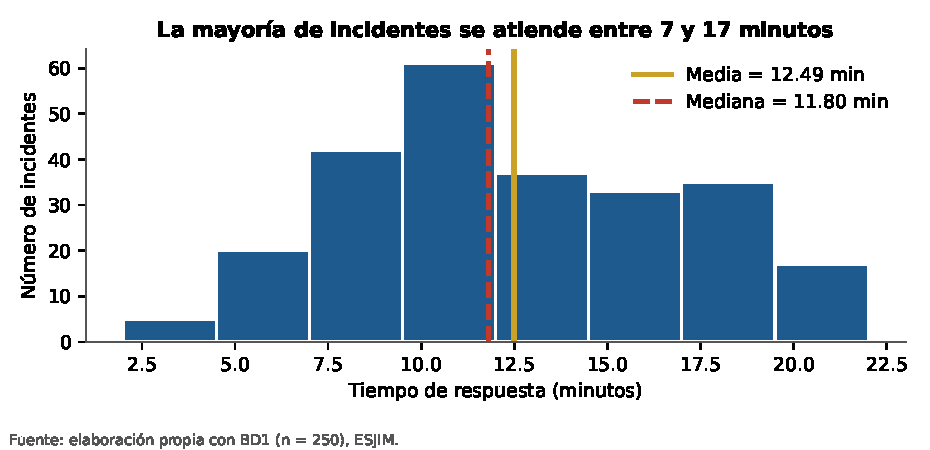
\includegraphics[width=0.86\textwidth]{fig/f1_histograma_tr.pdf}\\[-2pt]
{\footnotesize\textbf{Figura 1.} Histograma del tiempo de respuesta con media y mediana.}
\end{minipage}\end{center}

\textbf{Cómo leerlo.} La clase modal es 9,5--12 minutos (24,4 \% de los casos). El
20,8 \% de los incidentes ---los de las dos últimas clases--- se atiende en más de 17
minutos: ese grupo es el que conviene caracterizar (¿qué localidades?, ¿qué franjas?).

% ---------------- M3
\subsection{Modelo 3 --- Frecuencias por categoría y diagrama de Pareto}

\begin{cajaModelo}[Para qué sirve]
Ordenar categorías (tipo de delito, localidad, arma) de mayor a menor y acumular su
porcentaje. El principio de Pareto busca las pocas categorías que explican la mayor parte
de los casos, para priorizar.
\end{cajaModelo}

\textbf{En Excel:} tabla dinámica con \var{Tipo\_Delito} en filas y cuenta de
\var{ID\_Caso} en valores; ordenar descendente; columna de \% acumulado; gráfico
combinado (barras $+$ línea en eje secundario) o \textit{Insertar $\rightarrow$ Gráfico
estadístico $\rightarrow$ Pareto}.

\begin{center}\begin{minipage}{\linewidth}\centering
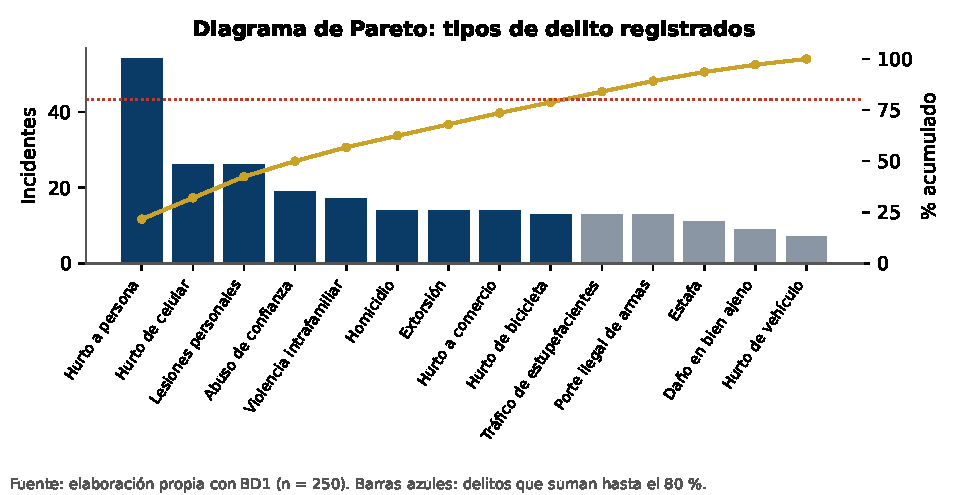
\includegraphics[width=0.9\textwidth]{fig/f2_pareto_delitos.pdf}\\[-2pt]
{\footnotesize\textbf{Figura 2.} Pareto de los 14 tipos de delito de BD1.}
\end{minipage}\end{center}

\textbf{Cómo leerlo.} El hurto a persona es la categoría más frecuente (54 casos,
21,6 \%), seguida por hurto de celular y lesiones personales (26 cada uno). Llegar al
80 \% exige \textbf{diez} de los catorce tipos de delito: en esta muestra el delito está
\textbf{repartido}, no concentrado en dos o tres categorías. Esa es una conclusión
válida y útil: obliga a priorizar por otro criterio (gravedad, tiempo de respuesta o
territorio) y no solo por frecuencia.

% ---------------- M4
\subsection{Modelo 4 --- Indicadores operativos y tasas}

\begin{cajaModelo}[Para qué sirve]
Convertir conteos en indicadores comparables entre unidades de distinto tamaño. Comparar
totales brutos entre ciudades o localidades con diferente número de registros o de
habitantes lleva a conclusiones falsas.
\end{cajaModelo}

\begin{gather*}
\text{Tasa por 10.000 hab.}=\frac{\text{delitos}}{\text{población}}\times 10.000
\qquad
\text{Costo por captura}=\frac{\text{costo operativo}}{\text{capturas}}\\[4pt]
\%\ \text{no atendidos}=\frac{\text{incidentes no atendidos}}{\text{llamadas al 123}}\times 100
\end{gather*}

\textbf{Ejemplo resuelto --- BD2 por ciudad}

\begin{center}
\small
\begin{tabular}{@{}lrrrrr@{}}
\toprule
Ciudad & Registros & Llamadas 123 & \% no atendidos & TR medio (min) & Costo por captura (COP)\\
\midrule
Bogotá & 100 & 1.097 & 24,5 & 9,97 & 671.723\\
Medellín & 68 & 645 & 23,9 & 8,72 & 628.301\\
Cali & 42 & 481 & 25,6 & 8,85 & 850.995\\
Barranquilla & 40 & 342 & 24,0 & 8,57 & 869.449\\
\bottomrule
\end{tabular}
\end{center}

\textbf{Cómo leerlo.} Cerca de \textbf{uno de cada cuatro} llamados al 123 queda sin
atender en las cuatro ciudades (628 de 2.565 en total, 24,5 \%). Bogotá tiene el mayor
tiempo medio de respuesta (9,97 min), pero un costo por captura menor que Cali y
Barranquilla. Por turno, la tarde recibe en promedio 12,05 llamadas frente a 8,42 en el
turno de día: \textbf{43,1 \% más demanda}, un dato clave para el plan de la Parte II.

% ---------------- M5
\subsection{Modelo 5 --- Probabilidad clásica y condicional}

\begin{cajaModelo}[Para qué sirve]
Estimar qué tan probable es un resultado (por ejemplo, la captura) y si esa probabilidad
cambia cuando se conoce una condición (el medio empleado, la franja, la localidad).
\end{cajaModelo}

\[
P(A)=\frac{\text{casos favorables}}{\text{casos posibles}}
\qquad
P(A\mid B)=\frac{P(A\cap B)}{P(B)}=\frac{n(A\cap B)}{n(B)}
\]
\textbf{En Excel:} tabla dinámica con \var{Arma\_Medio} en filas, \var{Captura} en
columnas y cuenta de casos (tabla de contingencia); luego dividir cada celda entre el
total de su fila.

\textbf{Ejemplo resuelto --- BD1, captura según el medio empleado}

\begin{center}
\small
\begin{tabular}{@{}lccc@{}}
\toprule
Medio empleado & Casos & Con captura & $P(\text{captura}\mid\text{medio})$\\
\midrule
Arma de fuego & 38 & 11 & 0,289\\
Contundente & 33 & 8 & 0,242\\
Arma blanca & 69 & 14 & 0,203\\
Sin arma & 81 & 14 & 0,173\\
Medios virtuales & 15 & 0 & 0,000\\
\midrule
Total de la base & 250 & 47 & 0,188\\
\bottomrule
\end{tabular}
\end{center}

\begin{center}\begin{minipage}{\linewidth}\centering
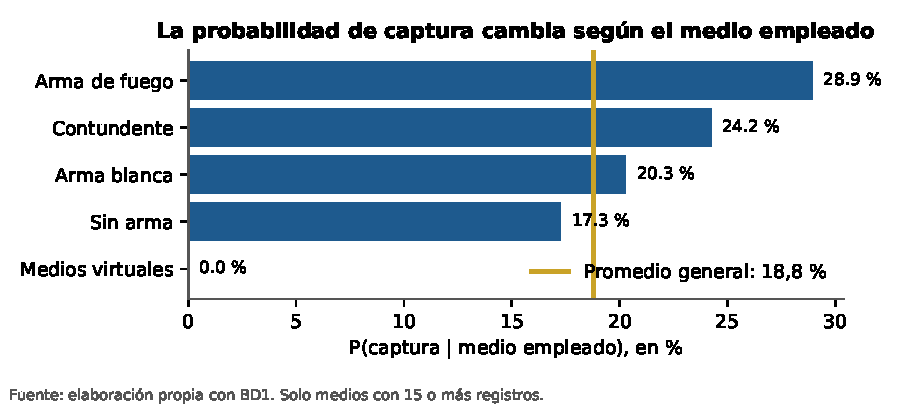
\includegraphics[width=0.84\textwidth]{fig/f3_prob_condicional.pdf}\\[-2pt]
{\footnotesize\textbf{Figura 3.} Probabilidad condicional de captura por medio empleado.}
\end{minipage}\end{center}

\textbf{Cómo leerlo.} La probabilidad general de captura es 0,188. Cuando el hecho
involucra arma de fuego sube a 0,289 (11 de 38), y en los 15 casos con medios virtuales
no hubo ninguna captura. Con muestras pequeñas (menos de 30 casos) presente la cifra con
prudencia: indica una tendencia, no una certeza.

% ---------------- M6
\subsection{Modelo 6 --- Distribución de Poisson}

\begin{cajaModelo}[Para qué sirve]
Modelar el número de veces que ocurre un evento en un intervalo (hurtos por mes, llamadas
por hora) y calcular la probabilidad de cada conteo. Permite fijar \textbf{umbrales de
alerta}: si un mes supera lo esperable, algo cambió en el territorio.
\end{cajaModelo}

\[
P(X=k)=\frac{e^{-\lambda}\,\lambda^{k}}{k!},\qquad k=0,1,2,\ldots
\qquad\text{con media}=\text{varianza}=\lambda
\]
\textbf{En Excel:} \var{=POISSON.DIST(k; lambda; FALSO)} para $P(X=k)$ y
\var{=POISSON.DIST(k; lambda; VERDADERO)} para $P(X\le k)$.

\textbf{Ejemplo resuelto --- BD1, hurto a persona por mes.} Hay 54 hurtos en 18 meses,
luego $\lambda = 54/18 = 3{,}0$ hurtos por mes.

\begin{center}
\small
\begin{tabular}{@{}ccccc@{}}
\toprule
$k$ & $P(X=k)$ & $P(X\le k)$ & Meses esperados ($18\cdot P$) & Meses observados\\
\midrule
0 & 0,050 & 0,050 & 0,90 & 1\\
1 & 0,149 & 0,199 & 2,69 & 1\\
2 & 0,224 & 0,423 & 4,03 & 6\\
3 & 0,224 & 0,647 & 4,03 & 2\\
4 & 0,168 & 0,815 & 3,02 & 5\\
5 & 0,101 & 0,916 & 1,81 & 3\\
6 & 0,050 & 0,967 & 0,91 & 0\\
7 o más & 0,034 & 1,000 & 0,60 & 0\\
\bottomrule
\end{tabular}
\end{center}

\begin{center}\begin{minipage}{\linewidth}\centering
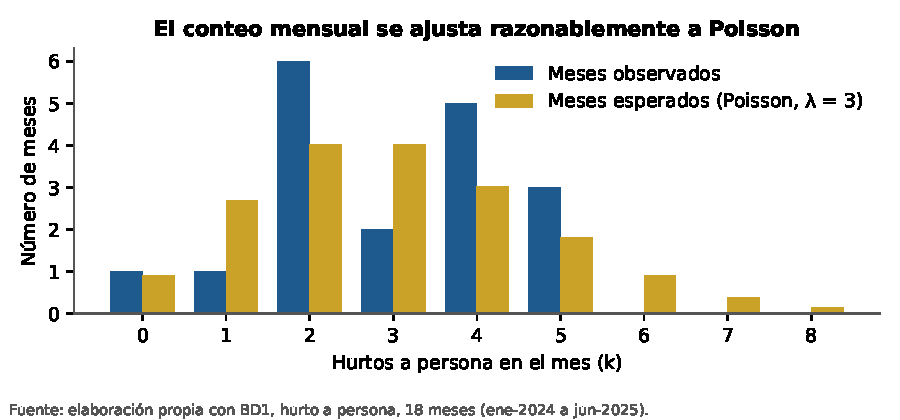
\includegraphics[width=0.84\textwidth]{fig/f4_poisson.pdf}\\[-2pt]
{\footnotesize\textbf{Figura 4.} Frecuencias observadas y esperadas según Poisson ($\lambda=3$).}
\end{minipage}\end{center}

\textbf{Validación del modelo.} La varianza de los conteos mensuales es 2,12, cercana a
la media (3,0). La prueba de dispersión
$\chi^2=\dfrac{(n-1)\,s^2}{\bar{x}}=\dfrac{17\times 2{,}12}{3{,}0}=12{,}0$ con 17 grados
de libertad da $p=0{,}80>0{,}05$: no hay sobredispersión y Poisson es adecuado
(\var{=PRUEBA.CHI.INV} o \var{=DISTR.CHICUAD.CD(12;17)}).

\textbf{Cómo leerlo.} Lo más probable es un mes con 2 o 3 hurtos (22,4 \% cada uno). La
probabilidad de 5 o más es 18,5 \%. Como $P(X\le 6)=0{,}967$, \textbf{un mes con 7 o
más hurtos a persona} tiene menos de 5 \% de probabilidad: es la señal objetiva para
revisar qué cambió.

% ---------------- M7
\subsection{Modelo 7 --- Correlación y regresión lineal}

\begin{cajaModelo}[Para qué sirve]
Medir si dos variables numéricas se mueven juntas (coeficiente de Pearson $r$) y
cuantificar cuánto cambia una cuando la otra aumenta una unidad (recta de regresión).
\end{cajaModelo}

\[
\hat{y}=a+b\,x,\qquad
b=\frac{\sum (x_i-\bar{x})(y_i-\bar{y})}{\sum (x_i-\bar{x})^2},\qquad
a=\bar{y}-b\,\bar{x},\qquad R^2=r^2
\]
\textbf{En Excel:} \var{=COEF.DE.CORREL()}, \var{=PENDIENTE()}, \var{=INTERSECCION.EJE()},
\var{=COEFICIENTE.R2()}, o \textit{Análisis de datos $\rightarrow$ Regresión} (entrega
además el valor $p$).

\textbf{Ejemplo resuelto --- BD2, patrullas disponibles ($x$) y tiempo de respuesta ($y$)}

\[
\hat{y}=12{,}08-1{,}48\,x,\qquad r=-0{,}44,\qquad R^2=0{,}195,\qquad p<0{,}001
\]

\begin{center}\begin{minipage}{\linewidth}\centering
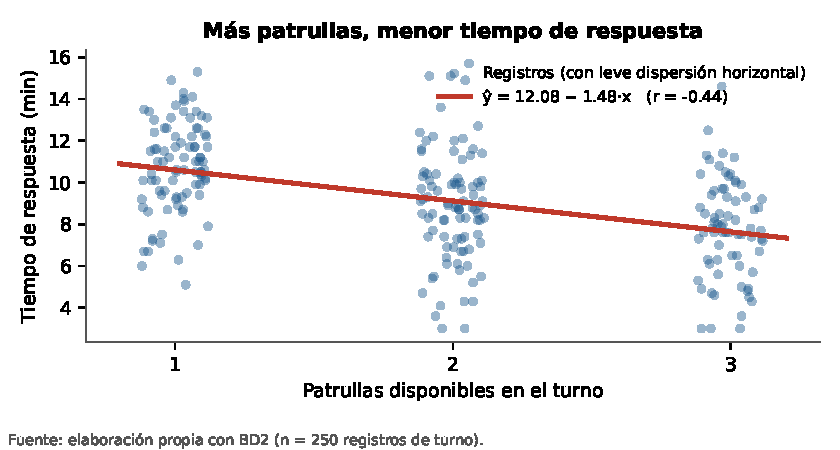
\includegraphics[width=0.78\textwidth]{fig/f5_regresion.pdf}\\[-2pt]
{\footnotesize\textbf{Figura 5.} Diagrama de dispersión y recta de regresión (BD2).}
\end{minipage}\end{center}

\textbf{Cómo leerlo.} La relación es \textbf{negativa y moderada}: con una patrulla el
tiempo medio es 10,73 min; con dos, 8,86; con tres, 7,80. Cada patrulla adicional se
asocia con \textbf{1,48 minutos menos} de respuesta. El $R^2=0{,}195$ indica que las
patrullas explican cerca del 20 \% de la variación; el resto depende de otros factores.
Si se agrega el área del cuadrante (regresión múltiple:
$\hat{y}=8{,}54-1{,}42\,\text{Patrullas}+1{,}83\,\text{Área}$), el $R^2$ sube a 0,32.

\begin{cajaAlerta}
\textbf{Errores frecuentes.} (1) Llamar ``moderada'' a una correlación de 0,98: por
encima de 0,8 en valor absoluto es \textbf{muy fuerte}; entre 0,4 y 0,6, moderada.
(2) Afirmar causalidad: la regresión muestra asociación; que más patrullas
\textit{causen} menos tiempo requiere otros elementos de juicio.
\end{cajaAlerta}

% ---------------- M8
\subsection{Modelo 8 --- Optimización de recursos}

La consigna pide ``aplicar técnicas de optimización para determinar la mejor
distribución de recursos policiales en función de la incidencia delictiva''. Se
presentan dos niveles; el segundo es el que distingue un trabajo sobresaliente.

\subsubsection*{8a. Reparto proporcional (método del mayor residuo)}

\[
\text{cuota}_i=\frac{d_i}{\sum d_j}\times R
\]
donde $d_i$ es la demanda de la unidad $i$ y $R$ el total de recursos. Se asigna la parte
entera de cada cuota y las unidades sobrantes se entregan a los mayores residuos decimales.

\textbf{Ejemplo --- repartir 30 policías entre cinco estaciones de Bogotá (BD2) según el
promedio de llamadas al 123 por turno.}

\begin{center}
\small
\begin{tabular}{@{}lccc@{}}
\toprule
Estación & Llamadas por turno ($d_i$) & Cuota exacta & Policías asignados\\
\midrule
Ciudad Bolívar & 15,18 & 8,49 & 8\\
Kennedy & 13,45 & 7,52 & 8\\
Engativá & 9,36 & 5,23 & 5\\
Suba & 9,30 & 5,20 & 5\\
Usaquén & 6,38 & 3,56 & 4\\
\midrule
Total & 53,67 & 30,00 & 30\\
\bottomrule
\end{tabular}
\end{center}
Las partes enteras suman 28; las dos unidades restantes van a Usaquén (residuo 0,56) y
Kennedy (0,52). Es transparente, pero considera un solo criterio.

\subsubsection*{8b. Programación lineal entera con Solver}

\begin{cajaInfo}[\textbf{Situación}]
El comando de Bogotá dispone de \textbf{6 patrullas adicionales por turno} para cinco
estaciones. Según la regresión del Modelo 7, cada patrulla reduce el tiempo de respuesta
en $b=1{,}48$ min. Se quiere \textbf{minimizar el tiempo de respuesta ponderado por la
demanda}, con la meta de que ninguna estación supere 10 minutos y con máximo 2 patrullas
adicionales por estación.
\end{cajaInfo}

\begin{cajaPaso}[\textbf{Paso 1 --- Variables de decisión}]
$x_i$ = patrullas adicionales asignadas a la estación $i$ (Ciudad Bolívar, Kennedy,
Engativá, Suba, Usaquén). Enteras y no negativas.
\end{cajaPaso}

\begin{cajaPaso}[\textbf{Paso 2 --- Función objetivo}]
Con $L_i$ = llamadas por turno y $T_i$ = tiempo actual:
\[
\min Z=\sum_{i=1}^{5} L_i\,(T_i-1{,}48\,x_i)
\quad\Longleftrightarrow\quad
\max\ \sum_{i=1}^{5} 1{,}48\,L_i\,x_i
\]
\end{cajaPaso}

\begin{cajaPaso}[\textbf{Paso 3 --- Restricciones}]
\[
\begin{aligned}
&x_1+x_2+x_3+x_4+x_5 = 6 && \text{(patrullas disponibles)}\\
&T_i-1{,}48\,x_i \le 10 && \text{(meta de 10 min en cada estación)}\\
&0\le x_i\le 2,\quad x_i\ \text{entero} && \text{(capacidad de cada estación)}
\end{aligned}
\]
La meta obliga a Suba ($T=10{,}99$) y Usaquén ($T=11{,}29$) a recibir al menos una
patrulla: $x_4\ge (10{,}99-10)/1{,}48=0{,}67\Rightarrow x_4\ge 1$ y
$x_5\ge 0{,}87\Rightarrow x_5\ge 1$.
\end{cajaPaso}

\begin{cajaPaso}[\textbf{Paso 4 --- Resolver con Solver}]
Celdas cambiantes: $x_1,\ldots,x_5$. Celda objetivo: \var{=SUMAPRODUCTO(L;T)-1,48*SUMAPRODUCTO(L;X)}
(minimizar). Restricciones: suma $=6$; tiempos nuevos $\le 10$; $x_i\le 2$; $x_i$
\textit{entero}. Método: \textit{Simplex LP}. (\textit{Datos $\rightarrow$ Solver}; si no
aparece, actívelo en \textit{Opciones $\rightarrow$ Complementos}.)
\end{cajaPaso}

\begin{center}
\small
\begin{tabular}{@{}lccccc@{}}
\toprule
Estación & $L_i$ & $T_i$ actual & $x_i^{*}$ & $T_i$ nuevo & ¿Cumple 10 min?\\
\midrule
Ciudad Bolívar & 15,18 & 9,32 & 2 & 6,36 & Sí\\
Kennedy & 13,45 & 9,11 & 2 & 6,15 & Sí\\
Engativá & 9,36 & 9,53 & 0 & 9,53 & Sí\\
Suba & 9,30 & 10,99 & 1 & 9,51 & Sí\\
Usaquén & 6,38 & 11,29 & 1 & 9,81 & Sí\\
\midrule
\multicolumn{3}{@{}l}{Tiempo ponderado por demanda} & & \multicolumn{2}{l}{9,83 $\rightarrow$ \textbf{7,81 min} ($-20{,}5$ \%)}\\
\bottomrule
\end{tabular}
\end{center}

\begin{center}\begin{minipage}{\linewidth}\centering
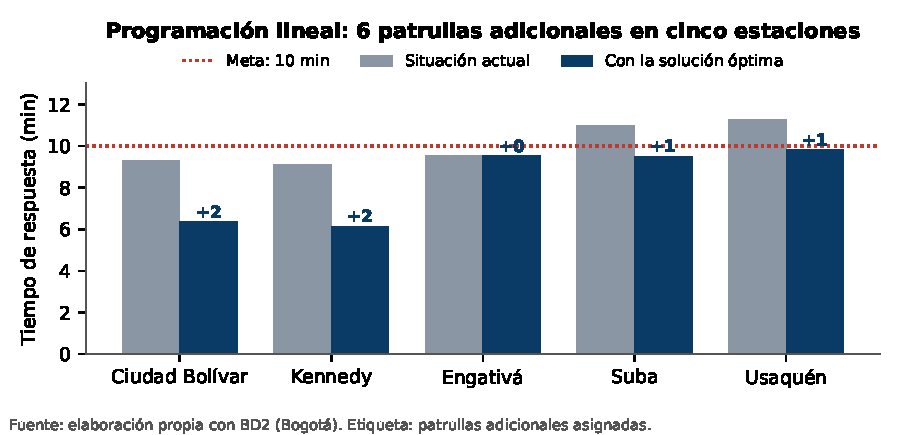
\includegraphics[width=0.84\textwidth]{fig/f6_programacion_lineal.pdf}\\[-2pt]
{\footnotesize\textbf{Figura 6.} Tiempo de respuesta antes y después de la asignación óptima.}
\end{minipage}\end{center}

\textbf{Cómo leerlo.} Sin la meta, el modelo llevaría todas las patrullas a las
estaciones con más llamadas. La restricción de 10 minutos \textbf{cambia la solución}:
obliga a atender a Suba y Usaquén aunque tengan menos demanda. Esa es la interpretación
que se espera: qué decide el modelo y por qué. \textbf{Verifique siempre} que la
solución cumple todas las restricciones que usted mismo planteó.

\begin{cajaExito}
\textbf{Otras formulaciones válidas de optimización.} Repartir personal para
\textit{maximizar la dotación mínima por incidente} (modelo max--min); minimizar el costo
operativo (\var{Costo\_Operativo\_COP}) cumpliendo un mínimo de incidentes atendidos;
asignar patrullas a franjas horarias según la demanda por turno. Escoja la que responda a
la pregunta de su grupo.
\end{cajaExito}

% ---------------- M9
\subsection{Modelo 9 --- Distribución binomial}

\begin{cajaModelo}[Para qué sirve]
Calcular la probabilidad de obtener $k$ ``éxitos'' en $n$ ensayos independientes con la
misma probabilidad $p$: capturas en un grupo de casos, llamadas atendidas a tiempo,
procedimientos exitosos.
\end{cajaModelo}

\[
P(X=k)=\binom{n}{k}p^{k}(1-p)^{n-k},\qquad E(X)=n\,p
\]
\textbf{En Excel:} \var{=DISTR.BINOM.N(k; n; p; FALSO)} y \var{=DISTR.BINOM.N(k; n; p; VERDADERO)}.

\textbf{Ejemplo resuelto --- BD1.} Con $p=0{,}188$ (tasa de captura de la base), ¿qué
esperar en los próximos 10 incidentes?

\begin{center}\begin{minipage}{\linewidth}\centering
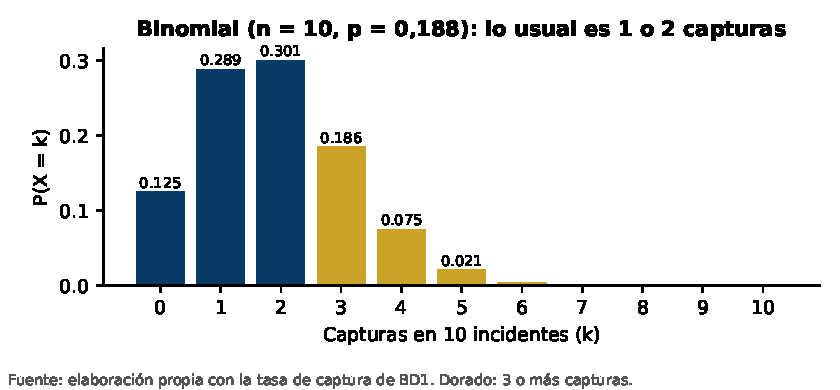
\includegraphics[width=0.74\textwidth]{fig/f8_binomial.pdf}\\[-2pt]
{\footnotesize\textbf{Figura 7.} Distribución binomial de capturas en 10 incidentes.}
\end{minipage}\end{center}

\textbf{Cómo leerlo.} Se esperan $E(X)=10\times 0{,}188=1{,}88$ capturas. La probabilidad
de no capturar a nadie es 0,125; la de al menos una, 0,875; la de tres o más, 0,286. Si
una estación logra 5 capturas en 10 casos ($P=0{,}021$), su resultado está muy por encima
de lo esperable: vale la pena documentar qué hizo distinto.

% ---------------- M10
\subsection{Modelo 10 --- Intervalos de confianza}

\begin{cajaModelo}[Para qué sirve]
Toda cifra calculada con una muestra tiene un margen de error. El intervalo de confianza
dice entre qué valores está, con 95 \% de confianza, el valor verdadero. Presentarlo
muestra ``precisión'' en el análisis.
\end{cajaModelo}

\[
\text{Proporción: } \hat{p}\pm 1{,}96\sqrt{\frac{\hat{p}(1-\hat{p})}{n}}
\qquad\qquad
\text{Media: } \bar{x}\pm t_{0{,}975;\,n-1}\,\frac{s}{\sqrt{n}}
\]
\textbf{En Excel:} \var{=INTERVALO.CONFIANZA.T(0,05; s; n)} entrega el margen de error de la media.

\textbf{Ejemplo resuelto --- BD1 ($n=250$).}
\begin{itemize}[leftmargin=1.4em,itemsep=1pt]
\item Tasa de captura: $0{,}188\pm 1{,}96\times 0{,}0247 \Rightarrow$ \textbf{entre 14,0 \% y 23,6 \%}.
\item Tiempo medio de respuesta: $12{,}49\pm 1{,}97\times 0{,}277 \Rightarrow$ \textbf{entre 11,95 y 13,04 minutos}.
\end{itemize}

\textbf{Cómo leerlo.} Decir ``la tasa de captura es 18,8 \%'' es incompleto: con 250 casos
el valor real podría estar entre 14 \% y 24 \%. Si una meta propone pasar de 18,8 \% a
20 \%, ese cambio cabe dentro del margen de error y no demostraría una mejora real.

% ---------------- M11
\subsection{Modelo 11 --- Prueba chi-cuadrado de independencia}

\begin{cajaModelo}[Para qué sirve]
Probar si dos variables categóricas están relacionadas o son independientes; por
ejemplo, si haber participado en un programa de resocialización se asocia con reincidir
menos.
\end{cajaModelo}

\[
\chi^2=\sum\frac{(O-E)^2}{E},\qquad E=\frac{\text{total de fila}\times\text{total de columna}}{n},\qquad gl=(f-1)(c-1)
\]
\textbf{En Excel:} \var{=PRUEBA.CHICUAD(rango observado; rango esperado)} devuelve el valor $p$.

\textbf{Ejemplo resuelto --- BD3, resocialización y reincidencia}

\begin{center}
\small
\begin{tabular}{@{}lccc|cc@{}}
\toprule
& No reincidió & Reincidió & Total & Esperado (reincidió) & \% reincidencia\\
\midrule
Sin programa & 77 & 78 & 155 & 70,06 & 50,3 \%\\
Con programa & 60 & 35 & 95 & 42,94 & 36,8 \%\\
\midrule
Total & 137 & 113 & 250 & & 45,2 \%\\
\bottomrule
\end{tabular}
\end{center}

$\chi^2=4{,}32$ con 1 grado de libertad; $p=0{,}038<0{,}05$.

\textbf{Cómo leerlo.} Se rechaza la independencia: quienes participaron en
resocialización reincidieron \textbf{13,5 puntos porcentuales menos} (36,8 \% frente a
50,3 \%). Es una asociación estadísticamente significativa; para afirmar que el programa
\textit{causa} la reducción habría que descartar que los participantes ya tuvieran
menor riesgo.

% ---------------- M12
\subsection{Modelo 12 --- Comparación de medias: prueba $t$ y ANOVA}

\begin{cajaModelo}[Para qué sirve]
Decidir si la diferencia entre los promedios de dos o más grupos es real o se debe al
azar del muestreo: tiempo de respuesta entre ciudades, turnos o estaciones.
\end{cajaModelo}

\textbf{Fórmula (ANOVA de un factor).} $F=\dfrac{\text{variabilidad entre grupos}}{\text{variabilidad dentro de los grupos}}$; si $p<0{,}05$, al menos una media es diferente.
\textbf{En Excel:} \textit{Análisis de datos $\rightarrow$ Análisis de varianza de un factor}; para dos grupos, \var{=PRUEBA.T(rango1; rango2; 2; 3)}.

\textbf{Ejemplo resuelto --- BD2, tiempo de respuesta por ciudad}

\begin{center}
\small
\begin{tabular}{@{}lccc@{}}
\toprule
Ciudad & $n$ & Media (min) & Desviación (min)\\
\midrule
Bogotá & 100 & 9,97 & 2,66\\
Cali & 42 & 8,85 & 2,29\\
Medellín & 68 & 8,72 & 2,64\\
Barranquilla & 40 & 8,57 & 2,79\\
\bottomrule
\end{tabular}
\end{center}
ANOVA: $F=4{,}72$; $p=0{,}003$. Prueba $t$ (Bogotá frente a las demás): $t=3{,}72$; $p<0{,}001$.

\begin{center}\begin{minipage}{\linewidth}\centering
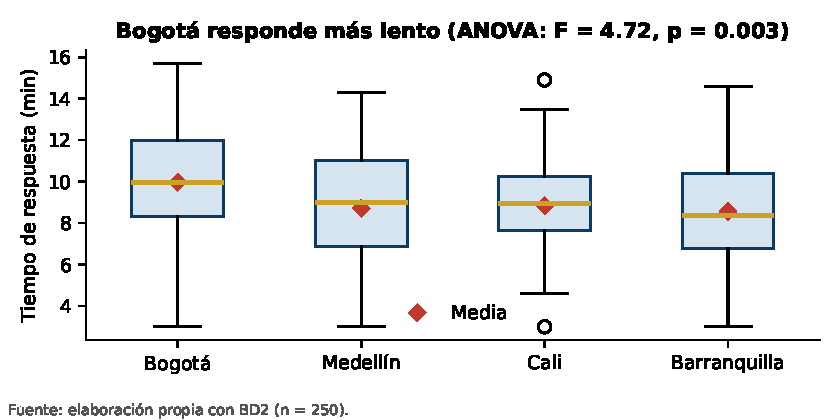
\includegraphics[width=0.74\textwidth]{fig/f9_anova.pdf}\\[-2pt]
{\footnotesize\textbf{Figura 8.} Diagrama de caja del tiempo de respuesta por ciudad.}
\end{minipage}\end{center}

\textbf{Cómo leerlo.} Bogotá tarda en promedio 1,2 a 1,4 minutos más que las otras tres
ciudades y la diferencia es estadísticamente significativa. Entre Cali, Medellín y
Barranquilla las diferencias son pequeñas. El diagrama de caja muestra además que las
dispersiones son parecidas.

% ---------------- M13
\subsection{Modelo 13 --- Regresión logística}

\begin{cajaModelo}[Para qué sirve]
Estimar la probabilidad de un resultado sí/no (reincidir, capturar) a partir de varias
variables a la vez, y medir cuánto aumenta o reduce cada una esa probabilidad mediante la
\textbf{razón de probabilidades} (OR, por sus siglas en inglés).
\end{cajaModelo}

\[
P(Y=1)=\frac{1}{1+e^{-(\beta_0+\beta_1x_1+\cdots+\beta_kx_k)}},\qquad OR_j=e^{\beta_j}
\]
\textbf{Herramientas:} Excel con Solver (maximizando la verosimilitud), JASP o jamovi
(gratuitos), R o Python.

\textbf{Ejemplo resuelto --- BD3, probabilidad de reincidir}

\begin{center}
\small
\begin{tabular}{@{}lccc@{}}
\toprule
Variable & OR & IC 95 \% & $p$\\
\midrule
Cada antecedente previo & 1,19 & 0,99 -- 1,42 & 0,059\\
Pertenece a banda & 1,75 & 1,03 -- 2,97 & 0,037\\
Participó en resocialización & 0,51 & 0,30 -- 0,88 & 0,016\\
Consume sustancias & 1,44 & 0,85 -- 2,42 & 0,172\\
Tenía empleo & 0,99 & 0,58 -- 1,71 & 0,973\\
\bottomrule
\end{tabular}
\end{center}

\begin{center}\begin{minipage}{\linewidth}\centering
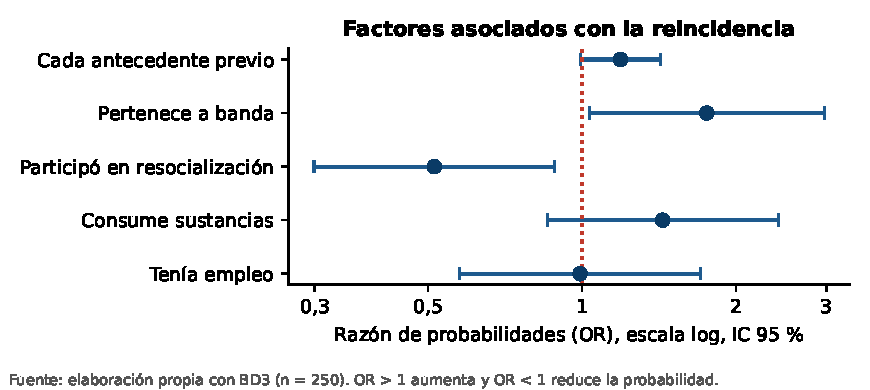
\includegraphics[width=0.74\textwidth]{fig/f10_logistica.pdf}\\[-2pt]
{\footnotesize\textbf{Figura 9.} Razones de probabilidades e intervalos de confianza.}
\end{minipage}\end{center}

\textbf{Cómo leerlo.} Manteniendo constantes las demás variables, pertenecer a una banda
multiplica por 1,75 las probabilidades relativas de reincidir y participar en
resocialización las reduce casi a la mitad (OR = 0,51). El empleo previo no muestra
efecto. Para un perfil con 3 antecedentes, que pertenece a banda, consume sustancias y no
tenía empleo, la probabilidad estimada es \textbf{0,69}; si además participa en
resocialización baja a \textbf{0,54}. El modelo acierta en el 62,8 \% de los casos y su
pseudo-$R^2$ es bajo (0,04): orienta, pero no sirve para decidir sobre una persona en
particular.

% ---------------- M14
\subsection{Modelo 14 --- Series de tiempo: tendencia y promedio móvil}

\begin{cajaModelo}[Para qué sirve]
Analizar cómo cambia una variable mes a mes: si hay tendencia (sube o baja), si hay
estacionalidad y cuánto esperar en los próximos periodos.
\end{cajaModelo}

\[
\text{Tendencia: } \hat{y}_t=a+b\,t
\qquad\qquad
\text{Promedio móvil de 3 meses: } \hat{y}_{t+1}=\frac{y_t+y_{t-1}+y_{t-2}}{3}
\]
\textbf{En Excel:} \var{=PRONOSTICO.LINEAL()}, \var{=TENDENCIA()}, \var{=PROMEDIO()} sobre
ventanas de 3 celdas, o \textit{Datos $\rightarrow$ Previsión}.

\textbf{Ejemplo resuelto --- BD1, incidentes por mes (ene-2024 a jun-2025)}

Serie: 7, 12, 17, 19, 9, 16, 12, 14, 19, 12, 21, 14, 16, 9, 14, 8, 15, 16 (media 13,9).
Tendencia: $\hat{y}_t=13{,}40+0{,}05\,t$, con $r=0{,}07$ y $p=0{,}78$.

\begin{center}\begin{minipage}{\linewidth}\centering
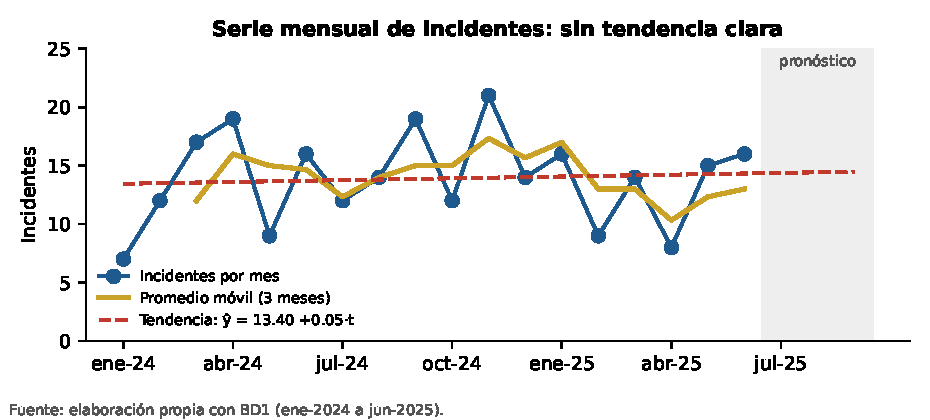
\includegraphics[width=0.82\textwidth]{fig/f11_serie.pdf}\\[-2pt]
{\footnotesize\textbf{Figura 10.} Serie mensual, promedio móvil y recta de tendencia.}
\end{minipage}\end{center}

\textbf{Cómo leerlo.} La pendiente (0,05 incidentes por mes) no es significativa: la
serie \textbf{no tiene tendencia}, oscila alrededor de 14 casos. El pronóstico por
promedio móvil para julio de 2025 es $(14+15+16)/3\approx 13$ incidentes. Con solo 18
meses no se puede afirmar estacionalidad; se necesitarían al menos dos o tres años.

% ---------------- M15
\subsection{Modelo 15 --- Teoría de colas M/M/c}

\begin{cajaModelo}[Para qué sirve]
Modelar un sistema en el que llegan solicitudes (llamadas al 123) y hay $c$ servidores
(patrullas) que las atienden. Permite calcular cuántas patrullas se necesitan para que la
espera no supere un límite.
\end{cajaModelo}

\textbf{Parámetros.} $\lambda$ = llegadas por hora; $\mu$ = atenciones por hora de cada
patrulla; $\rho=\lambda/(c\,\mu)$ = ocupación (debe ser menor que 1). La probabilidad de
esperar y la espera media $W_q$ se obtienen con la fórmula de Erlang C (disponible en
calculadoras en línea o en una hoja de Excel).

\textbf{Ejemplo resuelto --- BD2, Bogotá, turno de tarde.} Se reciben en promedio 12,97
llamadas en 8 horas: $\lambda=1{,}62$ por hora. \textbf{Supuesto:} cada atención toma 45
minutos, $\mu=1{,}33$ por hora (dato que el grupo debe justificar o ajustar).

\begin{center}
\small
\begin{tabular}{@{}ccccc@{}}
\toprule
Patrullas $c$ & Ocupación $\rho$ & P(la llamada espera) & Espera media $W_q$ & Llamadas en cola $L_q$\\
\midrule
2 & 61 \% & 46,0 \% & 26,4 min & 0,71\\
3 & 41 \% & 14,6 \% & 3,7 min & 0,10\\
4 & 30 \% & 3,9 \% & 0,6 min & 0,02\\
5 & 24 \% & 0,9 \% & 0,1 min & 0,00\\
\bottomrule
\end{tabular}
\end{center}

\textbf{Cómo leerlo.} Pasar de 2 a 3 patrullas reduce la espera media de 26,4 a 3,7
minutos; la cuarta patrulla aporta mucho menos (de 3,7 a 0,6). Ese es el punto de
\textbf{rendimientos decrecientes}: con 3 patrullas por cuadrante en la tarde se logra la
mayor parte de la mejora.

% ---------------- M16
\subsection{Modelo 16 --- Simulación Monte Carlo}

\begin{cajaModelo}[Para qué sirve]
Cuando un problema tiene incertidumbre, se simulan miles de escenarios aleatorios con
las distribuciones observadas y se mide con qué frecuencia ocurre cada resultado. Sirve
para comparar alternativas antes de aplicarlas.
\end{cajaModelo}

\textbf{En Excel:} \textit{Datos $\rightarrow$ Análisis de datos $\rightarrow$ Generación de
números aleatorios}, distribución \textit{Poisson} con $\lambda=12{,}05$ y 10.000 filas.
En la columna siguiente, \var{=MAX(0; demanda - capacidad)} da los casos sin atender de
cada turno; con \var{=CONTAR.SI()} y \var{=PROMEDIO()} se resumen los resultados.

\textbf{Ejemplo resuelto --- BD2, turno de tarde.} La demanda por turno sigue una Poisson
con media 12,05 llamadas; cada patrulla atiende 4 incidentes por turno (mediana
observada en la base). Se simularon 10.000 turnos:

\begin{center}
\small
\begin{tabular}{@{}cccc@{}}
\toprule
Patrullas & Capacidad (incidentes) & Turnos con casos sin atender & Demanda no atendida\\
\midrule
2 & 8 & 84,6 \% & 34,8 \%\\
3 & 12 & 42,5 \% & 11,5 \%\\
4 & 16 & 10,4 \% & 2,1 \%\\
\bottomrule
\end{tabular}
\end{center}

\begin{center}\begin{minipage}{\linewidth}\centering
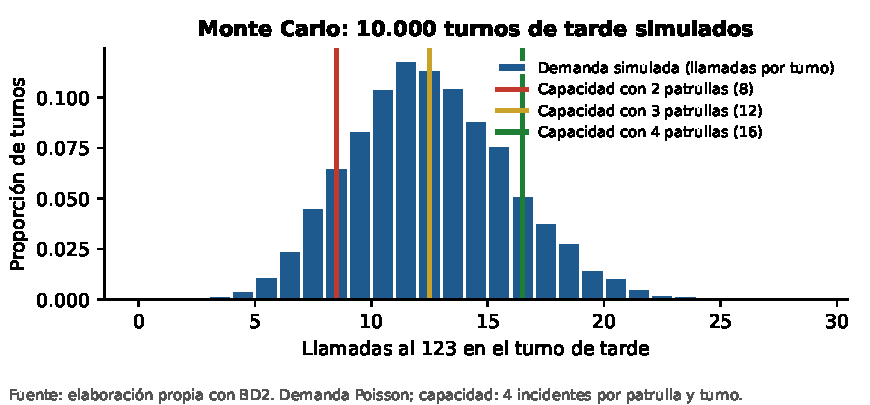
\includegraphics[width=0.78\textwidth]{fig/f12_montecarlo.pdf}\\[-2pt]
{\footnotesize\textbf{Figura 11.} Demanda simulada y capacidad según el número de patrullas.}
\end{minipage}\end{center}

\textbf{Cómo leerlo.} Con 2 patrullas, en 85 de cada 100 tardes quedarían casos sin
atender. Con 4, el riesgo baja a 10 de cada 100 y la demanda no atendida a 2 \%. La
simulación confirma lo que sugieren la teoría de colas y la regresión: el turno de tarde
necesita más vehículos que los otros.

% ---------------- M17
\subsection{Modelo 17 --- Agrupamiento K-Means (focos geográficos)}

\begin{cajaModelo}[Para qué sirve]
Agrupar incidentes según su cercanía geográfica (\var{Latitud}, \var{Longitud}) para
identificar focos o ``puntos calientes'' sin trazar zonas a mano.
\end{cajaModelo}

\textbf{Procedimiento.} (1) Elegir el número de grupos $k$; (2) ubicar $k$ centroides;
(3) asignar cada punto al centroide más cercano; (4) recalcular los centroides y repetir
hasta que no cambien. El $k$ se elige con el \textbf{coeficiente de silueta} (más alto,
mejor separados). \textbf{Herramientas:} JASP, jamovi, Python o R; en Excel puede
aproximarse con Solver minimizando la suma de distancias.

\textbf{Ejemplo resuelto --- BD1.} La silueta crece de 0,47 ($k=3$) a 0,56 ($k=8$); se
eligió $k=8$.

\begin{center}
\small
\begin{tabular}{@{}clccc@{}}
\toprule
Foco & Localidad dominante & Incidentes & TR medio (min) & Tasa de captura\\
\midrule
1 & Rafael Uribe Uribe & 59 & 13,1 & 11,9 \%\\
2 & Suba & 44 & 11,5 & 25,0 \%\\
3 & Kennedy & 41 & 12,9 & 19,5 \%\\
4 & Ciudad Bolívar & 24 & 15,6 & 25,0 \%\\
5 & Fontibón & 24 & 12,0 & 29,2 \%\\
6 & Usaquén & 22 & 9,6 & 13,6 \%\\
7 & Chapinero & 20 & 9,9 & 5,0 \%\\
8 & Bosa & 16 & 15,4 & 25,0 \%\\
\bottomrule
\end{tabular}
\end{center}

\begin{center}\begin{minipage}{\linewidth}\centering
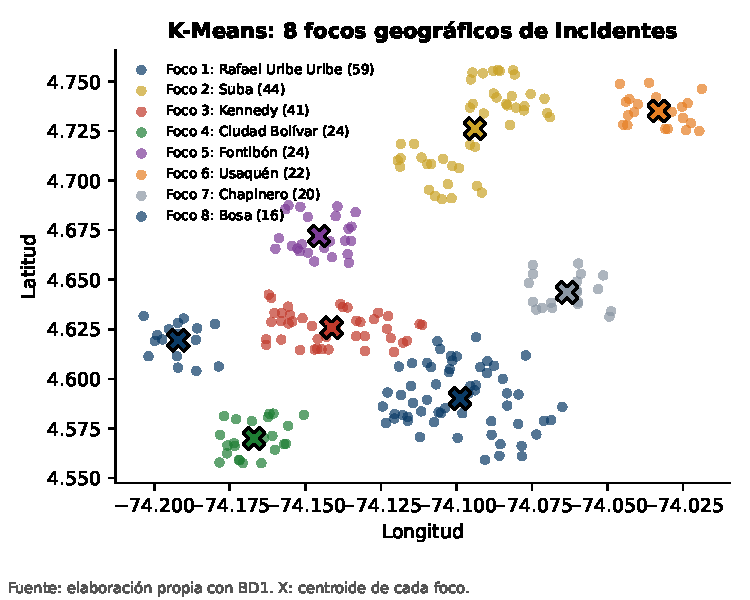
\includegraphics[width=0.62\textwidth]{fig/f13_kmeans.pdf}\\[-2pt]
{\footnotesize\textbf{Figura 12.} Focos geográficos identificados con K-Means.}
\end{minipage}\end{center}

\textbf{Cómo leerlo.} El foco más grande (59 incidentes) se centra en Rafael Uribe Uribe y
agrupa también casos de localidades vecinas; tiene una tasa de captura baja (11,9 \%).
Los focos de Ciudad Bolívar y Bosa combinan pocos casos con los tiempos de respuesta más
altos: allí la prioridad es la reacción, no la cantidad de patrullaje.

% ---------------- M18
\subsection{Modelo 18 --- Cadenas de Markov}

\begin{cajaModelo}[Para qué sirve]
Modelar cómo una persona o un sistema pasa de un estado a otro con ciertas
probabilidades (libre, capturado, en libertad con antecedentes, reincidente,
rehabilitado) y proyectar dónde estará después de varios periodos.
\end{cajaModelo}

\[
v_{t+1}=v_t\,P,\qquad v_t=v_0\,P^{t},\qquad \text{estado estable: } \pi=\pi P,\ \textstyle\sum\pi_i=1
\]
\textbf{En Excel:} \var{=MMULT(vector; matriz)} para avanzar un periodo; \var{=MMULT(matriz; matriz)} para $P^2$.

\textbf{Ejemplo resuelto --- BD3, hoja \textit{Matriz Transición (Ejemplo)}}

\begin{center}
\footnotesize
\begin{tabular}{@{}lccccc@{}}
\toprule
De $\backslash$ A & Libre s/a & Capturado 1.ª & Libertad c/a & Reincidente & Rehabilitado\\
\midrule
Libre sin antecedentes & 0,85 & 0,15 & 0 & 0 & 0\\
Capturado 1.ª vez & 0 & 0 & 0,70 & 0,10 & 0,20\\
Libertad con antecedentes & 0 & 0,25 & 0,35 & 0,25 & 0,15\\
Reincidente & 0 & 0,10 & 0,30 & 0,45 & 0,15\\
Rehabilitado & 0,60 & 0,05 & 0,15 & 0,05 & 0,15\\
\bottomrule
\end{tabular}
\end{center}

Para alguien capturado por primera vez ($v_0=(0,1,0,0,0)$): después de un periodo, 0,10
de probabilidad de ser reincidente; después de dos ($P^2$), \textbf{0,23}; después de tres
($P^3$), 0,21. A largo plazo (estado estable) la distribución es: libre 39,2 \%, capturado
13,6 \%, en libertad con antecedentes 23,4 \%, reincidente 14,0 \% y rehabilitado 9,8 \%.

\begin{center}\begin{minipage}{\linewidth}\centering
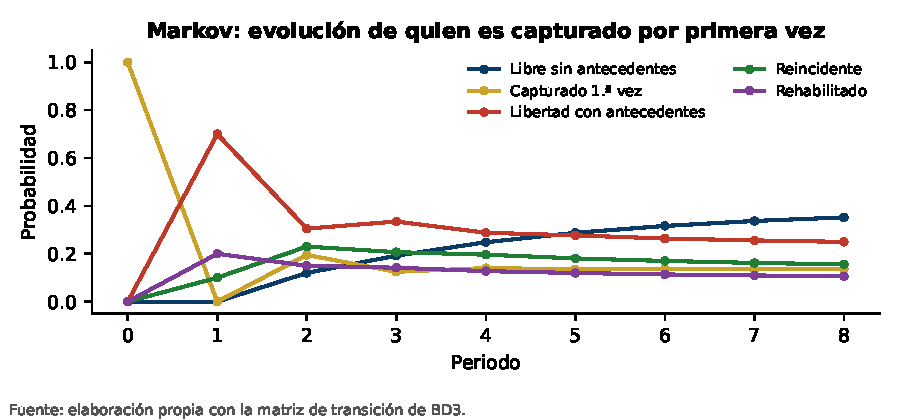
\includegraphics[width=0.8\textwidth]{fig/f14_markov.pdf}\\[-2pt]
{\footnotesize\textbf{Figura 13.} Evolución de las probabilidades de estado (Markov).}
\end{minipage}\end{center}

\textbf{Cómo leerlo.} El riesgo de reincidir se concentra en los dos primeros periodos
tras la primera captura (pico de 0,23): ahí deben actuar los programas de seguimiento.
La matriz de la base es un ejemplo didáctico; un grupo avanzado puede estimar su propia
matriz contando transiciones en la hoja \textit{Perfil y Reincidencia}.

% ---------------- resumen
\subsection{¿Qué modelo usar? Resumen del catálogo}

\begin{center}
\footnotesize
\begin{tabularx}{\textwidth}{@{}p{0.5cm}p{4.4cm}p{1.2cm}X@{}}
\toprule
& \textbf{Modelo} & \textbf{Base} & \textbf{Pregunta típica}\\
\midrule
1 & Tendencia central y dispersión & BD1 & ¿Cuál es el valor típico y qué tanto varía?\\
2 & Tabla de frecuencias e histograma & BD1 & ¿Cómo se distribuyen los valores?\\
3 & Pareto & BD1 & ¿Qué categorías concentran los casos?\\
4 & Indicadores y tasas & BD2 & ¿Cómo comparar unidades de distinto tamaño?\\
5 & Probabilidad condicional & BD1 & ¿Cambia la probabilidad según una condición?\\
6 & Poisson & BD1 & ¿Cuántos eventos esperar y cuándo alertar?\\
7 & Correlación y regresión lineal & BD2 & ¿Cuánto cambia una variable cuando la otra aumenta?\\
8 & Reparto proporcional y programación lineal & BD2 & ¿Cómo distribuir recursos limitados de forma óptima?\\
9 & Binomial & BD1 & ¿Cuántos éxitos esperar en $n$ casos?\\
10 & Intervalos de confianza & BD1 & ¿Qué tan precisa es mi cifra?\\
11 & Chi-cuadrado de independencia & BD3 & ¿Dos variables categóricas están relacionadas?\\
12 & Prueba $t$ y ANOVA & BD2 & ¿La diferencia entre grupos es real?\\
13 & Regresión logística & BD3 & ¿Qué factores aumentan la probabilidad de un resultado sí/no?\\
14 & Series de tiempo & BD1 & ¿Hay tendencia? ¿Cuánto esperar el próximo mes?\\
15 & Teoría de colas M/M/c & BD2 & ¿Cuántas patrullas para que la espera sea aceptable?\\
16 & Simulación Monte Carlo & BD2 & ¿Qué pasaría con cada alternativa bajo incertidumbre?\\
17 & K-Means & BD1 & ¿Dónde están los focos geográficos?\\
18 & Cadenas de Markov & BD3 & ¿Cómo evolucionan los estados de una persona en el tiempo?\\
\bottomrule
\end{tabularx}
\end{center}

\begin{cajaExito}
\textbf{Combinación recomendada para un informe sobresaliente.} Un modelo descriptivo
(1--4), uno de probabilidad o inferencia (5, 6, 9--12), uno de relación o predicción (7,
13, 14) y uno de decisión (8, 15, 16). Los modelos 17 y 18 suman valor en la Parte II
para localizar y anticipar los problemas.
\end{cajaExito}

% ===================================================== 5
\section{Representación gráfica: cómo lograr el 1,5}

El criterio de gráficos vale \textbf{1,5 puntos en ambas partes}: es tan importante como
el análisis. El nivel máximo pide gráficos ``de excelente calidad, correctamente
etiquetados y relevantes para el análisis''.

\begin{center}
\footnotesize
\begin{tabularx}{\textwidth}{@{}p{5cm}X@{}}
\toprule
\textbf{Si quiere mostrar\ldots} & \textbf{Use}\\
\midrule
La distribución de una variable numérica & Histograma (Figura 1) o diagrama de caja\\
Qué categorías pesan más & Barras ordenadas o Pareto (Figura 2)\\
Una probabilidad o tasa por grupo & Barras horizontales con línea de referencia (Figura 3)\\
Lo observado frente a un modelo & Barras agrupadas (Figura 4)\\
La relación entre dos variables & Diagrama de dispersión con recta (Figura 5)\\
El antes y el después de una decisión & Barras agrupadas con la meta marcada (Figura 6)\\
Diferencias entre grupos & Diagrama de caja (Figura 8)\\
Efecto de varios factores & Gráfico de razones de probabilidad con intervalos (Figura 9)\\
La evolución en el tiempo & Gráfico de líneas con tendencia y pronóstico (Figura 10)\\
Resultados de una simulación & Histograma con líneas de capacidad (Figura 11)\\
Ubicación geográfica y focos & Mapa de puntos por grupo (Figura 12) o Mapa 3D de Excel\\
Transiciones entre estados & Gráfico de líneas por estado (Figura 13)\\
Concentración en dos dimensiones (lugar $\times$ hora) & Mapa de calor (Figura 14)\\
\bottomrule
\end{tabularx}
\end{center}

\begin{cajaInfo}[\textbf{Siete reglas para cada figura}]
\begin{enumerate}[leftmargin=1.4em,itemsep=1pt]
\item Numerada (\textit{Figura 1}, \textit{Tabla 1}) y citada en el texto.
\item Título que \textbf{comunica el hallazgo}, no solo el tema: ``La tarde concentra 43 \% más llamadas'' es mejor que ``Llamadas por turno''.
\item Ejes con nombre y unidades (minutos, número de casos, \%).
\item Nota de fuente: ``Elaboración propia con BD1 (n = 250)''.
\item Hecha en Excel u otro software y exportada en buena resolución; \textbf{nunca} gráficos dibujados con caracteres de texto (bloques o rayas) ni capturas borrosas.
\item Un párrafo de interpretación debajo de cada figura: qué muestra y qué implica.
\item Solo las figuras que aporten: es mejor seis bien leídas que quince sin explicar.
\end{enumerate}
\end{cajaInfo}

% ===================================================== 6
\section{Estructura del informe de la Parte I (5 a 7 páginas)}

\begin{center}
\footnotesize
\begin{tabularx}{\textwidth}{@{}p{1.7cm}p{3.6cm}X@{}}
\toprule
\textbf{Página} & \textbf{Sección} & \textbf{Contenido mínimo}\\
\midrule
Portada & Datos institucionales & Escuela, asignatura y sección, título, \textbf{nombres de todos los integrantes}, docente, fecha.\\
1 & Introducción & Contexto policial, problema central, preguntas, objetivos.\\
2 & Datos & Base utilizada, $n$, periodo, variables seleccionadas y depuración.\\
3--5 & Modelos aplicados & Al menos tres modelos del catálogo, con fórmula, cálculo, tabla o figura e interpretación.\\
6 & Gráficos de apoyo & Figuras adicionales (mapa de calor, dispersión, mapa).\\
7 & Síntesis y paso a la Parte II & Hallazgos principales en cifras y qué se profundizará.\\
Final & Referencias & Normas APA, incluida la base de datos del aula.\\
\bottomrule
\end{tabularx}
\end{center}

% ===================================================== 7
\section{Parte II: de los resultados al plan operativo}

\subsection{Fase 1 --- Interpretar resultados y extraer patrones}

Un \textbf{patrón significativo} es una regularidad respaldada por una cifra y útil para
decidir. No es repetir el número: es decir qué significa. El nivel máximo del criterio
\textit{Interpretación de resultados} pide encontrar ``patrones significativos'' e
interpretarlos ``con precisión''.

\begin{center}
\footnotesize
\begin{tabularx}{\textwidth}{@{}p{0.5cm}XX@{}}
\toprule
& \textbf{Resultado (dato)} & \textbf{Patrón (qué significa para decidir)}\\
\midrule
P1 & TR medio de 15,7 min en San Cristóbal, 15,6 en Ciudad Bolívar y 15,4 en Bosa, frente a 9,6 en Usaquén (BD1) & La respuesta tarda 60 \% más en el sur: el problema es de reacción territorial, no de volumen.\\
P2 & 28 \% de los incidentes ocurre entre las 18:00 y las 24:00 (BD1) & La franja nocturna temprana es la de mayor carga.\\
P3 & La tarde recibe 43,1 \% más llamadas que el día (BD2) & La dotación debe crecer en la tarde, no repartirse igual en los tres turnos.\\
P4 & Hurto a persona: $\lambda=3$ por mes, 7 o más es anormal ($p<0{,}05$) & Existe un umbral objetivo para activar alertas.\\
P5 & Cada patrulla adicional: $-1{,}48$ min (BD2) & Reasignar vehículos tiene un efecto medible; la PL indica dónde.\\
P6 & 0 capturas en 15 casos con medios virtuales (BD1) & Estos delitos no se resuelven con patrullaje: requieren investigación especializada.\\
P7 & Con 2 patrullas la espera media en la tarde es 26,4 min; con 3, 3,7 min (colas, BD2) & La tercera patrulla en la tarde es la de mayor rendimiento.\\
P8 & Reincidencia de 36,8 \% con resocialización frente a 50,3 \% sin ella (BD3) & Los programas de seguimiento se asocian con menor reincidencia.\\
\bottomrule
\end{tabularx}
\end{center}

\begin{center}\begin{minipage}{\linewidth}\centering
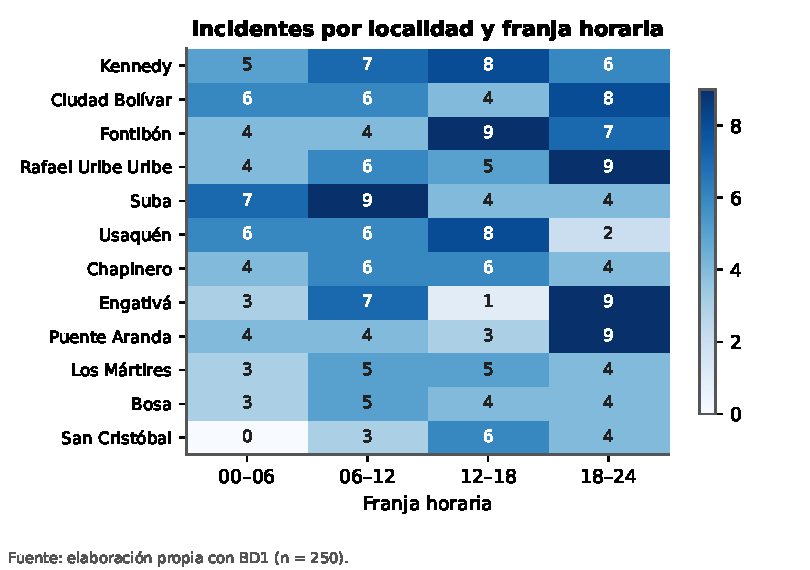
\includegraphics[width=0.66\textwidth]{fig/f7_mapa_calor.pdf}\\[-2pt]
{\footnotesize\textbf{Figura 14.} Mapa de calor de incidentes por localidad y franja horaria (BD1).}
\end{minipage}\end{center}

El mapa de calor ayuda a convertir patrones en acciones: Engativá, Puente Aranda y Rafael
Uribe Uribe registran 9 incidentes cada una entre las 18:00 y las 24:00; Fontibón, 9 entre
las 12:00 y las 18:00; Suba, 9 entre las 06:00 y las 12:00.

\subsection{Fase 2 --- Formular el plan operativo}

El plan es el \textbf{criterio distintivo de la Parte II}. El nivel máximo exige
``estrategias claras para optimizar recursos'' bien fundamentadas. Un plan con nivel
máximo responde, para cada acción, cinco preguntas: \textbf{qué} se hará, \textbf{con qué
dato} se justifica, \textbf{quién} lo hace, \textbf{cuándo} y \textbf{cómo se medirá}.

\begin{center}
\scriptsize
\begin{tabularx}{\textwidth}{@{}p{3.3cm}p{2.6cm}p{2.1cm}p{1.4cm}X@{}}
\toprule
\textbf{Acción} & \textbf{Fundamento} & \textbf{Responsable} & \textbf{Plazo} & \textbf{Indicador y meta}\\
\midrule
Asignar 2 patrullas adicionales a Ciudad Bolívar y Kennedy, y 1 a Suba y Usaquén & Solución de PL (Modelo 8b) & Planeación y comandantes de estación & Semana 2 & TR medio $\le$ 10 min en las cinco estaciones\\[3pt]
Reforzar el patrullaje de 18:00 a 24:00 en Engativá, Puente Aranda y Rafael Uribe Uribe & Mapa de calor (P2) & Jefes de turno & Semanas 2--8 & Incidentes en la franja: $-10$ \%\\[3pt]
Ubicar puntos de reacción en San Cristóbal, Bosa y Ciudad Bolívar & TR $>$ 15 min (P1) & Comandantes de estación & Semana 3 & \% de casos atendidos en $\le$ 15 min: de 70 \% a 85 \%\\[3pt]
Aumentar la dotación del turno de tarde & $+43{,}1$ \% de llamadas (P3) & Jefatura de servicio & Semana 2 & \% no atendidos: de 24,5 \% a 20 \%\\[3pt]
Alerta mensual por hurto a persona & Umbral de Poisson (P4) & Analista del CIEPS/SIEDCO & Mensual & Revisión obligatoria si $\ge$ 7 casos\\[3pt]
Remitir delitos con medios virtuales a policía judicial especializada & $P(\text{captura})=0$ (P6) & SIJIN & Semanas 1--8 & Casos con actuación investigativa\\[3pt]
Garantizar al menos 3 patrullas por cuadrante en el turno de tarde & Colas y Monte Carlo (P7) & Jefatura de servicio & Semana 2 & Demanda no atendida: de 34,8 \% a menos de 12 \%\\
\bottomrule
\end{tabularx}
\end{center}

\begin{cajaInfo}[\textbf{Cronograma sugerido}]
\textbf{Semana 1 --- Validar:} contrastar la propuesta con el pie de fuerza real, turnos y
mínimos de cobertura. \textbf{Semanas 2 a 7 --- Pilotear:} aplicar las acciones y registrar
los indicadores cada semana. \textbf{Semana 8 --- Evaluar:} comparar con la línea base,
revisar si el delito se desplazó a sectores vecinos y ajustar.
\end{cajaInfo}

\subsection{Fase 3 --- Conclusiones y recomendaciones}

\begin{cajaPaso}[\textbf{Conclusiones: una por pregunta de investigación, con su cifra}]
\textit{Débil:} ``La estadística es muy importante para la Policía''.\par
\textit{Bien fundamentada:} ``La asignación óptima de 6 patrullas reduce el tiempo de
respuesta ponderado de 9,83 a 7,81 minutos (20,5 \%) sin superar la meta de 10 minutos en
ninguna estación''.
\end{cajaPaso}

\begin{cajaPaso}[\textbf{Recomendaciones: accionables y con sus límites}]
Diga qué hacer para poner en marcha el plan (validar datos, pilotear, medir) y reconozca
los límites del análisis: la base es académica, la regresión muestra asociación y no
causalidad, y la decisión final corresponde al mando con información institucional.
\end{cajaPaso}

\subsection{Estructura del informe de la Parte II (8 a 10 páginas)}

\begin{center}
\footnotesize
\begin{tabularx}{\textwidth}{@{}p{1.7cm}p{3.6cm}X@{}}
\toprule
\textbf{Página} & \textbf{Sección} & \textbf{Contenido mínimo}\\
\midrule
Portada & Datos institucionales & Igual que en la Parte I.\\
1 & Introducción y contexto & Problema, preguntas y lo logrado en la Parte I.\\
2 & Datos y análisis & Retomado de la Parte I, corregido según la retroalimentación.\\
3--4 & Modelos aplicados & Retomados y mejorados; histograma, dispersión y tablas de frecuencia.\\
5--6 & Resultados & Patrones significativos (tabla tipo P1--P6) con sus figuras.\\
7--8 & Plan operativo & Matriz de acciones, responsables, plazos, indicadores y metas; cronograma.\\
9 & Conclusiones y recomendaciones & Una conclusión por pregunta; recomendaciones y límites.\\
Final & Referencias & Normas APA.\\
\bottomrule
\end{tabularx}
\end{center}

% ===================================================== 8
\section{Rúbricas de evaluación y cómo alcanzar el nivel máximo}

\subsection{Parte I}
\begin{center}
\scriptsize
\begin{tabularx}{\textwidth}{@{}p{2.2cm}p{0.6cm}XX@{}}
\toprule
\textbf{Criterio} & \textbf{Máx.} & \textbf{Nivel máximo (texto de la rúbrica)} & \textbf{Qué hacer para lograrlo}\\
\midrule
Análisis de datos & 1,5 & Interpreta con precisión los datos y aplica correctamente modelos matemáticos avanzados. & Trabajar con la base del aula; al menos tres modelos (uno descriptivo, uno probabilístico o de relación, uno de optimización); cálculos verificables e interpretación correcta.\\[3pt]
Representación gráfica & 1,5 & Gráficos y tablas de excelente calidad, correctamente etiquetados y relevantes para el análisis. & Seguir las siete reglas de la sección 5; cada figura con título que comunica, ejes, fuente e interpretación.\\[3pt]
Redacción y estructura & 1,0 & Excelente redacción y organización, con coherencia y cohesión. & Seguir la estructura de la sección 6; extensión de 5 a 7 páginas; revisar ortografía.\\[3pt]
Uso de herramientas estadísticas & 1,0 & Herramientas avanzadas de análisis con precisión y justificación. & Decir qué herramienta se usó y por qué (funciones de Excel, Análisis de datos, Solver); tabla pregunta--modelo--herramienta.\\
\bottomrule
\end{tabularx}
\end{center}
Niveles: criterios de 1,5 $\rightarrow$ 1,5 $\cdot$ 1,2 $\cdot$ 0,9 $\cdot$ 0,5 $\cdot$ 0;
criterios de 1,0 $\rightarrow$ 1,0 $\cdot$ 0,8 $\cdot$ 0,6 $\cdot$ 0,3 $\cdot$ 0.

\subsection{Parte II}
\begin{center}
\scriptsize
\begin{tabularx}{\textwidth}{@{}p{2.2cm}p{0.6cm}XX@{}}
\toprule
\textbf{Criterio} & \textbf{Máx.} & \textbf{Nivel máximo (texto de la rúbrica)} & \textbf{Qué hacer para lograrlo}\\
\midrule
Interpretación de resultados & 1,5 & Interpreta con precisión los resultados obtenidos y encuentra patrones significativos. & Tabla de patrones dato $\rightarrow$ significado; cifras coherentes con la Parte I.\\[3pt]
Representación gráfica & 1,5 & Gráficos y tablas de excelente calidad, correctamente etiquetados y relevantes. & Incluir histograma, diagrama de dispersión y tablas de frecuencia (los pide la consigna) más el gráfico del plan.\\[3pt]
Planificación, conclusiones y recomendaciones & 1,0 & Planificación y conclusiones bien fundamentadas, con estrategias claras para optimizar recursos. & Matriz acción--fundamento--responsable--plazo--indicador--meta; conclusiones con cifras; recomendaciones con límites.\\[3pt]
Redacción y estructura & 1,0 & Excelente redacción y organización, con coherencia y cohesión. & Estructura de la sección 7.4; extensión de 8 a 10 páginas.\\
\bottomrule
\end{tabularx}
\end{center}

% ===================================================== 9
\section{Errores que debe evitar}

Estos son los errores más frecuentes en las entregas revisadas. Cada uno resta puntos.

\begin{cajaAlerta}
\begin{enumerate}[leftmargin=1.4em,itemsep=2pt]
\item \textbf{Datos inventados o ``simulados''} en lugar de las bases del aula.
\item \textbf{Textos sobrantes de herramientas de inteligencia artificial}: ``sustituya estas cifras por las reales antes de entregar'', asteriscos de formato (\texttt{**}), restos como \texttt{html>}. Use las herramientas como apoyo, pero revise y haga suyo el documento.
\item \textbf{Gráficos dibujados con caracteres} o capturas de pantalla ilegibles.
\item \textbf{Interpretaciones invertidas}: sesgo, coeficiente de variación, fuerza de la correlación (véanse los Modelos 1 y 7).
\item \textbf{Cifras incoherentes}: decir que la muestra tiene 201 registros y calcular con 250; resultados que violan las restricciones planteadas.
\item \textbf{Mencionar un modelo sin aplicarlo}: ``se podría usar programación lineal'' o fórmulas en blanco no cuentan como modelo aplicado.
\item \textbf{Portada incompleta}: sin los nombres de todos los integrantes o con el nombre de otra asignatura.
\item \textbf{Extensión fuera de rango}: menos de 5 o más de 7 páginas (Parte I); menos de 8 o más de 10 (Parte II).
\item \textbf{Plan sin responsables, plazos ni indicadores}: una lista de buenas intenciones no es un plan operativo.
\item \textbf{Copiar el trabajo de otro grupo o de otra sección}: las entregas se comparan entre sí.
\end{enumerate}
\end{cajaAlerta}

% ===================================================== 10
\section{Lista de chequeo antes de entregar}

\begin{center}
\small
\begin{tabularx}{\textwidth}{@{}p{0.6cm}X p{1.2cm}p{1.2cm}@{}}
\toprule
& \textbf{Verificación} & \textbf{Parte I} & \textbf{Parte II}\\
\midrule
$\square$ & Portada con escuela, asignatura, sección, título, docente, fecha y nombres de todos los integrantes & \checkmark & \checkmark\\
$\square$ & Problema, preguntas y objetivos redactados & \checkmark & \checkmark\\
$\square$ & Base del aula identificada, con $n$ y periodo & \checkmark & \checkmark\\
$\square$ & Al menos tres modelos aplicados con cálculos e interpretación & \checkmark & \checkmark\\
$\square$ & Herramientas usadas declaradas y justificadas & \checkmark & \checkmark\\
$\square$ & Figuras numeradas, tituladas, con ejes, fuente e interpretación & \checkmark & \checkmark\\
$\square$ & Histograma, diagrama de dispersión y tabla de frecuencias & & \checkmark\\
$\square$ & Tabla de patrones significativos & & \checkmark\\
$\square$ & Plan operativo con acciones, responsables, plazos, indicadores y metas & & \checkmark\\
$\square$ & Conclusiones con cifras y recomendaciones con límites & & \checkmark\\
$\square$ & Sin textos sobrantes de herramientas de IA; ortografía revisada & \checkmark & \checkmark\\
$\square$ & Extensión dentro del rango; archivo en PDF & \checkmark & \checkmark\\
$\square$ & Cada integrante subió el archivo en su cuenta & \checkmark & \checkmark\\
\bottomrule
\end{tabularx}
\end{center}

% ===================================================== 11
\section{Recursos y referencias}

\subsection{Bases de datos y herramientas}
\begin{itemize}[leftmargin=1.4em,itemsep=1pt]
\item Escuela de Suboficiales y Nivel Ejecutivo ``Gonzalo Jiménez de Quesada''. (2026). \textit{BD1 Incidentes delictivos Bogotá; BD2 Gestión de cuadrantes Colombia; BD3 Perfil criminal y reincidencia} [Bases de datos académicas en Excel]. Aula virtual de Matemática aplicada a la profesión.
\item Microsoft Excel: funciones estadísticas, complemento \textit{Análisis de datos} y \textit{Solver}.
\item Grabaciones de los encuentros sincrónicos y material de clase de la Unidad 1 en el aula virtual.
\end{itemize}

\subsection{Bibliografía}
\begin{itemize}[leftmargin=1.4em,itemsep=1pt]
\item Hillier, F. S., \& Lieberman, G. J. (2015). \textit{Investigación de operaciones} (10.ª ed.). McGraw-Hill.
\item Triola, M. F. (2018). \textit{Estadística} (12.ª ed.). Pearson.
\item Walpole, R. E., Myers, R. H., Myers, S. L., \& Ye, K. (2012). \textit{Probabilidad y estadística para ingeniería y ciencias} (9.ª ed.). Pearson.
\item Chaiken, J. M., \& Dormont, P. (1978). A patrol car allocation model: Capabilities and algorithms. \textit{Management Science, 24}(12), 1291--1300.
\item Braga, A. A., Turchan, B. S., Papachristos, A. V., \& Hureau, D. M. (2019). Hot spots policing of small geographic areas effects on crime. \textit{Campbell Systematic Reviews, 15}(3), e1046.
\item Ratcliffe, J. H. (2016). \textit{Intelligence-led policing} (2.ª ed.). Routledge.
\item Policía Nacional de Colombia. (2024). \textit{Resolución 04341 de 2024, por la cual se define y regula el Modelo del Servicio de Policía Orientado a las Personas y los Territorios}.
\end{itemize}

\vspace{0.5cm}
\begin{cajaExito}
\textbf{Dudas.} Use el \textit{Foro de dudas} del aula o el \textit{Foro grupal} de su
equipo. Las preguntas que se hacen a tiempo evitan los errores de la sección 9.
\end{cajaExito}

\end{document}
